This section delves into the analysis of two distinct economic frameworks. In Section \ref{C3-SubSection:A-Limitation-of-AKS-style-Model}, the optimal drilling and extraction model developed in \cite{Hotelling-under-Pressure_AKS_2018} is reformulated by introducing heterogeneity in resource quality. And it is shown that the recast model cannot justify the empirically observed simultaneous drilling of well locations with varying quality levels. In the subsequent portions of this section, a continuous-time Discrete Choice Dynamic Programming (DCDP) model for oil and gas extraction is developed, successfully articulating the simultaneous drilling of horizontal wells with heterogeneous quality.

% A Limitation of AKS-style Model
\subsection{A Limitation of AKS-style Model}
\label{C3-SubSection:A-Limitation-of-AKS-style-Model}
The theoretical framework for optimal oil drilling and extraction delineated in \cite{Hotelling-under-Pressure_AKS_2018} (AKS) can be augmented by integrating heterogeneity in the quality of well locations. Suppose that the fracking firm owns well sites of different qualities, indexed by $g \in \{L(ow), H(igh)\}$, and that a homogeneous good (i.e., oil) is yielded from the sites in which new horizontal wells are drilled. Furthermore, suppose that the unit price of the output, $\widebar{p}$, is determined exogenously due to the firm's total production being negligible in comparison to the global market for the output. The maximization problem of the firm owning a continuum of infinitesimal well locations with disparate qualities can be articulated as follows:
\begin{equation}
\begin{split}
    \underset{d^{g}(t), \ g \in \{L, H\}}{\max} \hspace{0.2cm} \int_{0}^{\infty} e^{-rt} \left\{ \widebar{p} \sum_{g} \alpha^{g} d^{g}(t) \ - \ C\left( \sum_{g} d^{g}(t) \right) \right\} dt
\end{split}
\label{Equation:AKS-Style-Model_Objective-Function}
\end{equation}
subject to
%\begin{equation}
%\begin{split}
%    \dot{K}(t) \ = \ - \delta \sum_{g} q^{g}(t) \ + \ \sum_{g} I^{g} d^{g}(t), \hspace{0.3cm} K_{0} \ = \ K(0) \ \text{given,}
%\end{split}
%\end{equation}
\begin{equation}
\begin{split}
    \dot{R}^{g}(t) \ = \ - d^{g}(t), \hspace{0.3cm} R_{0}^{g} \ = \ R^{g}(0) \ \text{given,} 
\end{split}
\end{equation}
%\begin{equation}
%\begin{split}
%    q^{g}(t) \ \geq \ 0, \hspace{0.3cm} 0 \ \leq \ \sum_{g} q^{g}(t) \ \leq \ K(t),
%\end{split}
%\end{equation}
\begin{equation}
\begin{split}
    d^{g}(t) \ \geq \ 0, \hspace{0.3cm} R^{g}(t) \ \geq \ 0.
\end{split}
\end{equation}

In this formulation, state variables $R^{g}(t)$ denote the measure of undrilled well sites at a given time $t$. We simplify the AKS model by assuming that firms always produce at their production capacity constraint. This assumption reduces the complexity of the model. Control variables $d^{g}(t)$ represent the rate at which new horizontal wells are drilled at time $t$. $\alpha^{g}$ are the quantity of oil production from the marginally drilled well. Here, we assume that $\alpha^{H} > \alpha^{L}$. $C(\cdot)$, indicating the total instantaneous cost of drilling, is solely a function of the drilling rates.\footnote{Regarding the total cost of oil production, we follow the assumption made in \cite{Hotelling-under-Pressure_AKS_2018}: per-barrel extraction costs from existing wells are negligible.} Of note, in this formulation for $C(\cdot)$, we assume that locations are perfect substitutes on the cost side. And the profit obtained at time $t$ is discounted at the interest rate $r$.  

The current-value Hamiltonian-Lagrangian of the firm's problem is
\begin{equation}
\begin{split}
    \mathcal{H} \ 
    & = \ p(t) \sum_{g} q^{g}(t) \ - \ C\left( \sum_{g} d^{g}(t) \right) \\
    & \hspace{0.5cm} + \ \pi_{K}(t) \left\{ - \delta \sum_{g} q^{g}(t) \ + \sum_{g} I^{g} d^{g}(t) \right\} \\
    & \hspace{0.5cm} + \ \sum_{g} \pi_{R}^{g}(t) \left( -d^{g}(t) \right) \\ 
    & \hspace{0.5cm} + \ \sum_{g} \lambda_{1}^{g}(t) q^{g}(t) \ + \ \lambda_{2}(t) \sum_{g} q^{g}(t) \ + \ \lambda_{3}(t) \left\{ K(t) \ - \ \sum_{g} q^{g}(t) \right\} \\
    & \hspace{0.5cm} + \ \sum_{g} \lambda_{4}^{g}(t) d^{g}(t) \ + \ \sum_{g} \lambda_{5}^{g}(t) R^{g}(t),
\end{split}
\label{Equation:AKS-Style-Model_Current-Value-Hamiltonian}
\end{equation}

where $\pi^{g}_{R}$ are costate variables for the state variables $R^{g}$. $\lambda_{j}, \ j \in \{1, 2\}$ are the shadow cost of each constraint.

For a given quality level $g$, two necessary conditions characterize the firm's optimal rate of drilling:
\begin{equation}
\begin{split}
    d^{g}(t) \ \geq \ 0, \hspace{0.2cm} \alpha^{g} \widebar{p} \ - \ C'\left( \sum_{g} d^{g}(t) \right) \ - \ \pi^{g}(t) \ + \ \lambda_{1}^{g}(t) \ \leq \ 0, \hspace{0.2cm} C.S.,
\end{split}
\label{Equation:AKS-Style-Model_Necessary-Conditions_pi-K}
\end{equation}
\begin{equation}
\begin{split}
    \dot{\pi}^{g}(t) \ = \ r \pi^{g}(t) \ - \ \lambda_{2}^{g}(t).
\end{split}
\label{Equation:AKS-Style-Model_Necessary-Conditions_pi-R}
\end{equation}

When horizontal wells with heterogeneous quality are drilled simultaneously (i.e., for each $g$, $d^{g}(t) >0$, which leads to $\lambda_{1}^{g}(t) = 0$), necessary condition (\ref{Equation:AKS-Style-Model_Necessary-Conditions_pi-K}) implies that the shadow price on the resource constraint at time $t$ equals the profit on the marginal well:
\begin{equation}
\begin{split}
    \pi^{g} (t) \
    & = \ \alpha^{g} \widebar{p} \ - \ C'\left( \sum_{g} d^{g}(t) \right).
\end{split}
\label{Equation:AKS-Style-Model_Necessary-Conditions_Shadow-Price-pi}
\end{equation}

In addition, when both types of horizontal well sites are not fully exhausted (i.e., for each $g$, $R^{g}(t) > 0$, which in turn $\lambda_{2}^{g}(t) = 0$), necessary condition (\ref{Equation:AKS-Style-Model_Necessary-Conditions_pi-R}) means that the shadow value of the marginal undrilled well at time $t$ grows at the rate of $r$:
\begin{equation}
\begin{split}
    \dot{\pi}^{g} (t) \
    & = \ r \pi^{g} (t).
\end{split}
\label{Equation:AKS-Style-Model_Necessary-Conditions_Simplified-pi}
\end{equation}


The necessary conditions collectively suggest that the simultaneous drilling of horizontal wells with heterogeneous quality cannot be justified in the AKS framework when $d^{g}(t) > 0$ and $R^{g}(t) > 0$, which hold before all available well sites are developed.
The following stems from equation (\ref{Equation:AKS-Style-Model_Necessary-Conditions_Shadow-Price-pi}):
\begin{equation}
\begin{split}
    \pi^{H} (t) \ - \ \pi^{L} (t) \
    & = \ (\alpha^{H} - \alpha^{L}) \widebar{p}.
\end{split}
\label{Equation:AKS-Style-Model_Difference-between-pis}
\end{equation}

This relationship implies that the difference in the shadow value between high- and low-quality well locations is simply a revenue difference at any time $t$. And as shown below, differentiating equation (\ref{Equation:AKS-Style-Model_Necessary-Conditions_Shadow-Price-pi}) with respect to time implies that for a given $C'' (\cdot)$, $\dot{d}^{g} (t)$ and $d^{g} (t)$ determine the value of the time derivative of $\pi_{t}^{g} (t), \ g \in \{L, H\}$ and that $\dot{\pi}_{t}^{L} (t)$ and $\dot{\pi}_{t}^{H} (t)$ have the same value at a given time $t$:
\begin{equation}
\begin{split}
    \dot{\pi}^{L} (t), \ \dot{\pi}^{H} (t) \
    & = \ -\left( \sum_{g} \dot{d}^{g}(t) \right) C''\left( \sum_{g} d^{g}(t) \right).
\end{split}
\label{Equation:AKS-Style-Model_pi-dots}
\end{equation}

Here, based on equation (\ref{Equation:AKS-Style-Model_Necessary-Conditions_Simplified-pi}), the relationship between the time derivatives for two distinct qualities indicates that $\pi^{L} (t) = \pi^{H} (t)$ holds at all time $t$. However, this equality contradicts equation (\ref{Equation:AKS-Style-Model_Difference-between-pis}) because $\alpha^{H} > \alpha^{L}$. In other words, the simultaneous drilling of horizontal wells with heterogeneous quality does not hold in the AKS framework. 

Adding a constraint on extraction capacity, as is done in \cite{Extraction-Capacity-and-the-Optimal-Order-of-Extraction_Holland_2003}, can suggest that simultaneous extraction of different resource qualities is optimal. However, in the framework, setting the upper bound of an extraction-related constraint seems too arbitrary and complicates drawing implications from necessary conditions. From the empirical perspective, it is also intractable to quantify the margin for market-wide, or firm-wide, extraction capacity for each drilling decision. Furthermore, empirical estimation of the model from microeconomic data on drilling and production is, in general, too demanding. Those difficulties call for a new theoretical approach that thoroughly explains our empirical findings for drilling decisions made by fracking firms in North Dakota. 

The need leads us to develop a continuous-time Discrete Choice Dynamic Programming (DCDP) model that formulates a firm's drilling decision on a particular well site as an optimal stopping problem. Under this new theoretical framework, we can rationalize the simultaneous drilling of horizontal wells with heterogeneous resource quality without specifying any capacity constraint. Moreover, our DCDP model yields empirically testable predictions about how firms' drilling and production activities vary with oil prices. In the next section, we will present the basic elements and assumptions of our DCDP framework. 


% Setup
\subsection{Setup}
\label{C3-SubSection:Setup}
This section presents the basic elements and assumptions of our continuous-time Discrete Choice Dynamic Programming (DCDP) model that formulates fracking firms' drilling decisions on a particular well site as an optimal stopping problem. Following \cite{Hotelling-under-Pressure_AKS_2018}, we assume a continuum of infinitesimally small well sites in which horizontal wells will be drilled. Contrary to the AKS-style model, our DCDP model can rationalize the simultaneous drilling of horizontal wells with heterogeneous quality. Moreover, our theoretical framework yields predictions, being testable by utilizing detailed data on drilling and extraction in North Dakota, about how the frackers' drilling activity varies with oil prices. 

The state of a given well site at the beginning of time $t$ is represented by using a well-site-level state variable $s_{t}$ as follows:
\begin{equation}
    s_{t} \ = \ 
    \begin{cases}
        \ 0 \hspace{0.5cm} \text{when the well site has not been drilled yet} \\
        \ 1 \hspace{0.5cm} \text{when the well site is already drilled.}
    \end{cases}
\label{Equation:DCDP-Model_State-Variable}
\end{equation}

For a given well site that has not been developed, the firm makes a choice at time $t$ between two alternatives $a_{t} \in \{ 0, 1 \}$, which is a well-site-level control variable:
\begin{equation}
    a_{t} \ = \ 
    \begin{cases}
        \ 0 \hspace{0.5cm} \text{if the firm decides not to drill a well in the site} \\
        \ 1 \hspace{0.5cm} \text{if the firm decides to drill a well in the site.}
    \end{cases}
\label{Equation:DCDP-Model_Control-Variable}
\end{equation}
Intuitively, the two alternatives are constrained. To be specific, the constraint depends on the value of $s_{t}$:
\begin{equation}
    a_{t}(s_{t}) \ \in \ 
    \begin{cases}
        \ \{ 0, 1 \} \hspace{0.5cm} \text{when} \hspace{0.2cm} s_{t} = 0 \\ 
        \ \{ 0 \} \hspace{0.85cm} \text{when} \hspace{0.2cm} s_{t} = 1.
    \end{cases}
\label{Equation:DCDP-Model_Constraints-of-Control-Variable}
\end{equation}

The oil production from a horizontal well drilled at time $t$ is assumed to occur only during the very period:
\begin{equation}
\begin{split}
     q_{t} \ 
     & = \ \alpha a_{t},
\end{split}
\label{Equation:DCDP-Model_Oil-Production}
\end{equation}
where $\alpha$ is the amount of oil produced from a well. For simplicity, it is also assumed that $\alpha$ is a constant across well locations.

The marginal drilling-associated costs at time $t$ are assumed to be uniform across well sites.\footnote{As in Section \ref{C3-SubSection:A-Limitation-of-AKS-style-Model}, we take the assumption of the negligible extraction costs.} We also assume linear marginal costs of drilling a horizontal well. That is, 
\begin{equation}
\begin{split}
     c_{t} \
     & = \ c_{0} \ + \ c_{1} a_{t}.
\end{split}
\label{Equation:DCDP-Model_Cost}
\end{equation}

The oil price at time $t$, denoted $p_{t}$, is another state variable in our model. Regarding oil prices, two different scenarios are possible in our model. If the oil production industry is small relative to the world oil market, then $p_{t}$ is the world price $\bar{p}$. In other words, $p_{t}$ is exogenous. In the endogenous-price scenario, the market clearing $p_{t}$ is determined from a linear inverse demand curve:
\begin{equation}
\begin{split}
     p_{t} \ 
     & = \ p(Q_{t}) \\
     & = \ p_{0} \ - \ p_{1}Q_{t},
\end{split}
\label{Equation:DCDP-Model_Oil-Prices}
\end{equation}
where $Q_{t}$ is aggregate oil production, which will be described in detail later. 

Let $R_{t}$ denote the remaining level of well sites at time $t$. Suppose its initial level is normalized to 1 (i.e., $R_{0} = 1$).

For a given well location that has not been drilled before time $t$, the probability of drilling the well at time $t$ conditional on $s_{t}$ and $p_{t}$ can be defined as follows:
\begin{equation}
\begin{split}
     Pr_{t} \
     & \equiv \ \Pr \big( a_{t} = 1 | s_{t} = 0, p_{t} \big).
\end{split}
\label{Equation:DCDP-Model_Definition-of-CCP}
\end{equation}

Intuitively, aggregate drilling at time $t$ can be expressed with $R_{t}$ and $Pr_{t}$ as follows:
\begin{equation}
\begin{split}
     D_{t} \
     \equiv \ R_{t} Pr_{t}.
\end{split}
\label{Equation:DCDP-Model_Aggregate-Drilling}
\end{equation}
From this definition, the evolution path of the remaining well sites is governed by the following relationship:
\begin{equation}
\begin{split}
     \dot{R}_{t} \
     \equiv \ -D_{t} \hspace{0.2cm} (= -R_{t} Pr_{t}).
\end{split}
\label{Equation:DCDP-Model_Reserve}
\end{equation}
In addition, due to the assumption that $\alpha$ is uniform across well sites, the aggregate oil production $Q_{t}$ is proportional to $D_{t}$:
\begin{equation}
\begin{split}
     Q_{t} \
     \equiv \ \alpha D_{t} \ = \ \alpha \lambda_{a} R_{t} Pr_{t}.
\end{split}
\label{Equation:DCDP-Model_Aggregate-Oil-Production}
\end{equation}

The utility obtained from an individual well site can be represented by exploiting an additively separable utility function:
\begin{equation}
\begin{split}
     U(s_{t}, a_{t}, \epsilon_{t}) \ 
     & = \ \tilde{U}(s_{t}, a_{t}) \ + \ \epsilon(a_{t}) \\
     & = \ 
     \begin{cases}
          \ \epsilon_{0,t} \hspace{3.9cm} \text{if} \hspace{0.2cm} s_{t} = 0 \text{ and } a_{t} = 0 \\
          \ u(\alpha) \ - \ (c_{0} + c_{1}) \ + \ \epsilon_{1,t} \hspace{0.55cm} \text{if} \hspace{0.2cm} s_{t} = 0 \text{ and } a_{t} = 1 \\ 
          \ 0 \hspace{4.2cm} \text{if} \hspace{0.2cm} s_{t} = 1,
     \end{cases}
\end{split}
\label{Equation:DCDP-Model_Utility-Function}
\end{equation}
In the utility function, $\epsilon_{t}$ is idiosyncratic utility shocks at time $t$ that rely on the firm's choice at that time and are observable only to the firm. If the $\epsilon(a_{t})$'s follow the Type 1 Extreme Value (T1EV) distribution with the location parameter 0 and the scale parameter $\sigma$ and are I.I.D., then the expected value of $\epsilon(a_{t})$ conditional on the chosen alternative $a(t)$ is
\begin{equation}
\begin{split}
     e_{1t} \
     & \equiv \ E[\epsilon_{1t} \ | \ a_{t} = 1] \ = \ \sigma \left( \gamma \ - \ \ln (Pr_{t}) \right).
\end{split}
\label{Equation:DCDP-Model_Expected-Value-of-Epsilon}
\end{equation}
Here, $\gamma$ and $CCP(a_{t})$ are Euler's constant and the probability of choosing $a_{t}$ conditional on states at time $t$, respectively. For example, when $a_{t} = 1$, the utility shock's expected value is $\sigma \left( \gamma \ - \ \ln (Pr_{t}) \right)$. 


% Social Planner's Problem
\subsection{Social Planner's Problem and Necessary Conditions}
\label{C3-SubSection:Social-Planners-Problem-and-Necessary-Conditions}
In this section, using the continuous-time DCDP framework, we develop the social planner's problem. When an opportunity to drill potential well sites arrives, the social planner makes two decisions. First, the planner must choose, via the choice of $Pr_{t}$, the aggregate quantity of drilling. Second, the planner must also decide which locations will be drilled. Each site can be indexed by $\epsilon_{1t} - \epsilon_{0t}$, and so selecting which sites to drill can be thought of as selecting which indices to drill. Because there is a continuum of potential well locations, determining the optimal policy (i.e., the optimal $Pr_{t})$ is simply to choose a threshold that does not depend on the specific set of cost shocks realized at time $t$. Potential well locations with indices above the threshold drill, whereas those below it wait to drill. The one-to-one mapping between the threshold index and the choice of $Pr_{t}$ is characterized by equation (\ref{Equation:DCDP-Model_Decision-Rule}).

The goal of the social planner is to maximize welfare in the market. In this maximization problem, for a given $Pr_{t}$, the market's welfare obtained from potential well sites at time $t$ is defined as follows\footnote{Using $D_{t}$, we can re-write the definition: $W_{t}^{sp} \ = \ R_{t} f_{t} \ + \ u(\alpha D_{t}) \ - \ c(D_{t}) \ + \ D_{t} \sigma \big( \gamma \ - \ \ln(Pr_{t}) \big) \ + \ (\lambda_{a} R_{t} - D_{t}) \sigma \big( \gamma \ - \ \ln(1 - Pr_{t}) \big)$.}:
\begin{equation}
\begin{split}
     W_{t}^{sp} \ 
     & \equiv \ R_{t} f_{t} \\
     & \hspace{0.7cm} + \ u(\alpha \lambda_{a} R_{t} Pr_{t}) \ - \ c(\lambda_{a} R_{t} Pr_{t}) \\
     & \hspace{0.7cm} + \ \lambda_{a} R_{t} \Big\{ Pr_{t} \cdot \sigma \big( \gamma \ - \ \ln(Pr_{t}) \big) \ + \ (1 - Pr_{t}) \cdot \sigma \big( \gamma \ - \ \ln(1 - Pr_{t}) \big) \Big\}
\label{Equation:Social-Planners-Problem_Welfare}
\end{split}
\end{equation}
As shown, the welfare of the market at time $t$ consists of three components.\footnote{$W_{t}^{sp}$ can be interpreted differently. To be specific, $W_{t}^{sp}$ is the sum of the flow payoff from the undrilled well sites at time $t$ $\left( \text{i.e., } R_{t} f_{t} \right)$, the net (expected) payoff obtained from the marginally drilled well site at time $t$ $\left( \text{i.e., } u(\alpha \lambda_{a} R_{t} Pr_{t}) - c(\lambda_{a} R_{t} Pr_{t}) + \lambda_{a} R_{t} Pr_{t} \sigma \big( \gamma \ - \ \ln(Pr_{t}) \big) \right)$, and the (expected) gains from the well sites that are available but decided not to drill at time $t$ $\left( \text{i.e., } \lambda_{a} R_{t} (1 - Pr_{t}) \sigma \big( \gamma \ - \ \ln(1 - Pr_{t}) \big) \right)$.} The first line indicates the flow payoff received from undrilled well locations at time $t$. The second line means the choice-specific instantaneous payoff, which is presented as equation (\ref{Equation:DCDP-Model_Payoff-Function_Social-Planners-Problem}). The last line suggests the payoff related to choice-specific cost shocks.\footnote{The last line in equation (\ref{Equation:Social-Planners-Problem_Welfare}) can be rewritten using $e_{0}$ and $e_{1}$: \par \hspace{0.3cm} $\lambda_{a} R_{t} \big\{ Pr_{t} \cdot \sigma \big( \gamma \ - \ \ln(Pr_{t}) \big) \ + \ (1 - Pr_{t}) \cdot \sigma \big( \gamma \ - \ \ln(1 - Pr_{t}) \big) \big\} \ = \ \lambda_{a} R_{t} \big\{ Pr_{t} \cdot e_{1} \ + \ (1 - Pr_{t}) \cdot e_{0} \big\}$.} Note that regarding the choice-dependent cost shocks, their expected value is used and that only the terms in the last two lines, which depend on the social planner's drilling decisions, are associated with $\lambda_{a}$. 

In the continuous-time DCDP framework, the social planner's welfare problem is given by
\begin{footnotesize}
\begin{equation}
\begin{split}
     \underset{\{Pr_{t}\}_{t = 0}^{\infty}}{\max} \hspace{0.1cm} \int_{0}^{\infty} e^{-rt} \bigg[ u(\alpha R_{t} Pr_{t}) - c(R_{t} Pr_{t}) + R_{t} f_{t} + R_{t} \Big\{ Pr_{t} \cdot \sigma \big( \gamma - \ln(Pr_{t}) \big) + (1 - Pr_{t}) \cdot \sigma \big( \gamma - \ln(1 - Pr_{t}) \big) \Big\} \bigg] dt
\end{split}
\label{Equation:Social-Planners-Problem_Formulation}
\end{equation}
\end{footnotesize}
subject to
\begin{equation}
\begin{split}
    \dot{R}_{t} \ = \ -R_{t}Pr_{t} \ + \ E, \hspace{0.3cm} R_{0} \ = \ R(0) \ = \ 1 \hspace{0.2cm} \text{given,}
\end{split}
\label{Equation:Social-Planners-Problem_Law-of-Motion}
\end{equation}
\begin{equation}
\begin{split}
    R_{t} \ \geq \ 0, \hspace{0.3cm} 0 \ < \ Pr_{t} \ < \ 1.
\end{split}
\end{equation}
As shown, $W_{t}^{sp}$ is discounted at the rate of interest $r$. 

Under the assumption of an interior solution, the current-value Hamiltonian-Lagrangian of the social planner's problem is given by
\begin{equation}
\begin{split}
    \mathcal{H}^{sp} \ 
    & = \ R_{t} f_{t} \\
    & \hspace{0.7cm} + \ u(\alpha \lambda_{a} R_{t} Pr_{t}) \ - \ c(\lambda_{a} R_{t} Pr_{t}) \\
    & \hspace{0.7cm} + \ \lambda_{a} R_{t} \big\{ Pr_{t} \cdot \sigma \big( \gamma \ - \ \ln(Pr_{t}) \big) \ + \ (1 - Pr_{t}) \cdot \sigma \big( \gamma \ - \ \ln( 1 - Pr_{t}) \big) \big\} \\
    & \hspace{0.7cm} + \ \pi_{t} (-\lambda_{a} R_{t} Pr_{t} + E).
%    \ + \ \lambda_{1,t} (R_{t}) \ + \ \lambda_{2,t} (1 - Pr_{t}) \ + \ \lambda_{3,t} (Pr_{t}).
\end{split}
\label{Equation:Social-Planners-Problem_Hamiltonian-Lagrangian}
\end{equation}

The necessary conditions of the current-value Hamiltonian-Lagrangian are as follows:
\begin{equation}
\begin{split}
    & R_{t} \big\{ \alpha u'(\alpha R_{t} Pr_{t}) \ - \ c'(R_{t} Pr_{t}) \ - \ \sigma \ln(Pr_{t}) \ + \ \sigma \ln(1 - Pr_{t}) \ - \ \pi_{t} \big\} \ \leq \ 0, \hspace{0.2cm} Pr_{t} \ \geq \ 0,  \hspace{0.2cm} \text{C.S.}, \\
%    \ - \ \lambda_{2,t} \ + \ \lambda_{3,t} \ \leq \ 0, \\
%    & \hspace{0.5cm} Pr_{t} \ \geq \ 0,  \hspace{0.2cm} \text{C.S.},
\end{split}
\label{Equation:Social-Planners-Problem_Necessary-Conditions_Drilling-Probability}
\end{equation}
\begin{equation}
\begin{split}
    \dot{\pi}_{t} \ 
    & = \ r \pi_{t} \ - \ \left\{ f_{t} \ + \ \sigma \big( \gamma \ - \ \ln(1 - Pr_{t}) \big) \right\},
%     \ - \ \lambda_{1,t},
\end{split}
\label{Equation:Social-Planners-Problem_Necessary-Conditions_Costate-Variable}
\end{equation}
\begin{equation}
\begin{split}
    \lim_{t \rightarrow \infty} e^{-rt} (R_{t} \pi_{t}) \ = \ 0.
\end{split}
\label{Equation:Social-Planners-Problem_Transversality-Condition}
\end{equation}
If $R_{t} > 0$, necessary condition (\ref{Equation:Social-Planners-Problem_Necessary-Conditions_Drilling-Probability}) yields the following expression for the costate variable $\pi_{t}$, which is a function of $R_{t}$ and $Pr_{t}$:
\begin{equation}
\begin{split}
    \pi_{t} \ 
    & = \ \alpha u'(\alpha R_{t} Pr_{t}) \ - \ c'(R_{t} Pr_{t}) \ - \ \sigma \ln(Pr_{t}) \ + \ \sigma \ln(1 - Pr_{t}) \\
    & = \ \big\{ \alpha u'(\alpha R_{t} Pr_{t}) \ - \ c'(R_{t} Pr_{t}) \ + \ \sigma \big( \gamma \ - \ \ln(Pr_{t}) \big) \big\} \ - \ \sigma \big( \gamma \ - \ \ln(1 - Pr_{t}) \big).
\end{split}
\label{Equation:Social-Planners-Problem_Meaning-of-Costate-Variable}
\end{equation}
In addition, substituting condition (\ref{Equation:Social-Planners-Problem_Meaning-of-Costate-Variable}) into condition (\ref{Equation:Social-Planners-Problem_Necessary-Conditions_Costate-Variable}) yields the following Euler equation that governs the dynamics of the social planner's welfare maximization problem over time:
\begin{equation}
\begin{split}
    % \dot{\pi}_{t} \ 
    % & = \ r \pi_{t} \ - \ \sigma \big( \gamma \ + \  \ln(1 - Pr_{t}) \big) \\
    % (\dot{\pi}_{t} \ - \ r\pi_{t}) e^{-rt} \
    % & = \ - \sigma \big( \gamma \ - \ \ln(1 - Pr_{t}) \big) e^{-rt} \\
    % \pi_{t} e^{-rt} \
    % & = \ \int_{t}^{\infty} e^{-r\tau} \sigma \big( \gamma \ - \ \ln(1 - Pr_{\tau}) \big) d\tau \ + \ \mathcal{C} \\  % C = 0 from the equation for \pi_{t} at the steady state.
    \pi_{t} \
    & = \ e^{rt} \left[ \int_{t}^{\infty} e^{-r\tau} \Big\{ f_{t} \ + \ \sigma \big( \gamma \ - \ \ln(1 - Pr_{\tau}) \big) \Big\} d\tau \right],
\end{split}
\label{Equation:Social-Planners-Problem_Euler-Equation}
\end{equation}
We will discuss the implications of necessary conditions (\ref{Equation:Social-Planners-Problem_Necessary-Conditions_Costate-Variable}) and (\ref{Equation:Social-Planners-Problem_Meaning-of-Costate-Variable}) later. 

The social planner's problem has a unique steady state $(R_{ss}, \pi_{ss})$ such that $\dot{R}_{ss}, \ \dot{\pi}_{ss} = 0$. From necessary conditions (\ref{Equation:Social-Planners-Problem_Law-of-Motion}) and (\ref{Equation:Social-Planners-Problem_Necessary-Conditions_Costate-Variable}), $R_{t}$ and $\pi_{t}$ must satisfy the following equations at steady state:
\begin{equation}
    \begin{cases}
        \begin{split}
        \ R_{ss} \
        & = \ \frac{E}{ \ \lambda_{a} Pr_{ss} \ } \\
        \ \pi_{ss} \
        & = \ \frac{ \ f_{t} \ + \ \lambda_{a} \sigma \left( \gamma \ - \ \ln(1 - Pr_{ss}) \right) \ }{r}.
        \end{split}
    \end{cases}
\label{Equation:Social-Planners-Problem_System-of-Equations-for-Steady-State}
\end{equation}
On top of the equations, necessary condition (\ref{Equation:Social-Planners-Problem_Meaning-of-Costate-Variable}) has to hold at the steady state simultaneously. Solving the system of three equations, we can uniquely identify $(R_{ss}, \pi_{ss})$, including the value of the control variable at the steady state (i.e., $Pr_{ss}$). As implied by the first equation in (\ref{Equation:Social-Planners-Problem_System-of-Equations-for-Steady-State}), $R_{ss}$ is non-zero positive if $E \neq 0$. Using a Taylor series approximation, $\dot{R}_{t}$ and $\dot{\pi}_{t}$ can be linearized near the steady state $(R_{ss}, \pi_{ss})$, and this linearization process shows that the steady state of the infinite-horizon maximization problem is a saddle point, which is demonstrated in Figure \ref{Figure:Phase-Diagram_Saddle-Point}.\footnote{Regarding the saddle property, see \textit{9.5 Steady states in autonomous infinite-horizon problems} in \cite{Optimal-Control-Theory-and-Static-Optimization-in-Economics_Leonard-and-Long_1992}. And derivation details are provided in \ref{C3-Appendix_Derivations_Linearization-near-the-Steady-State-of-the-Social-Planners-Problem}.}
\afterpage{
    \begin{figure}[t!]
        \centering
        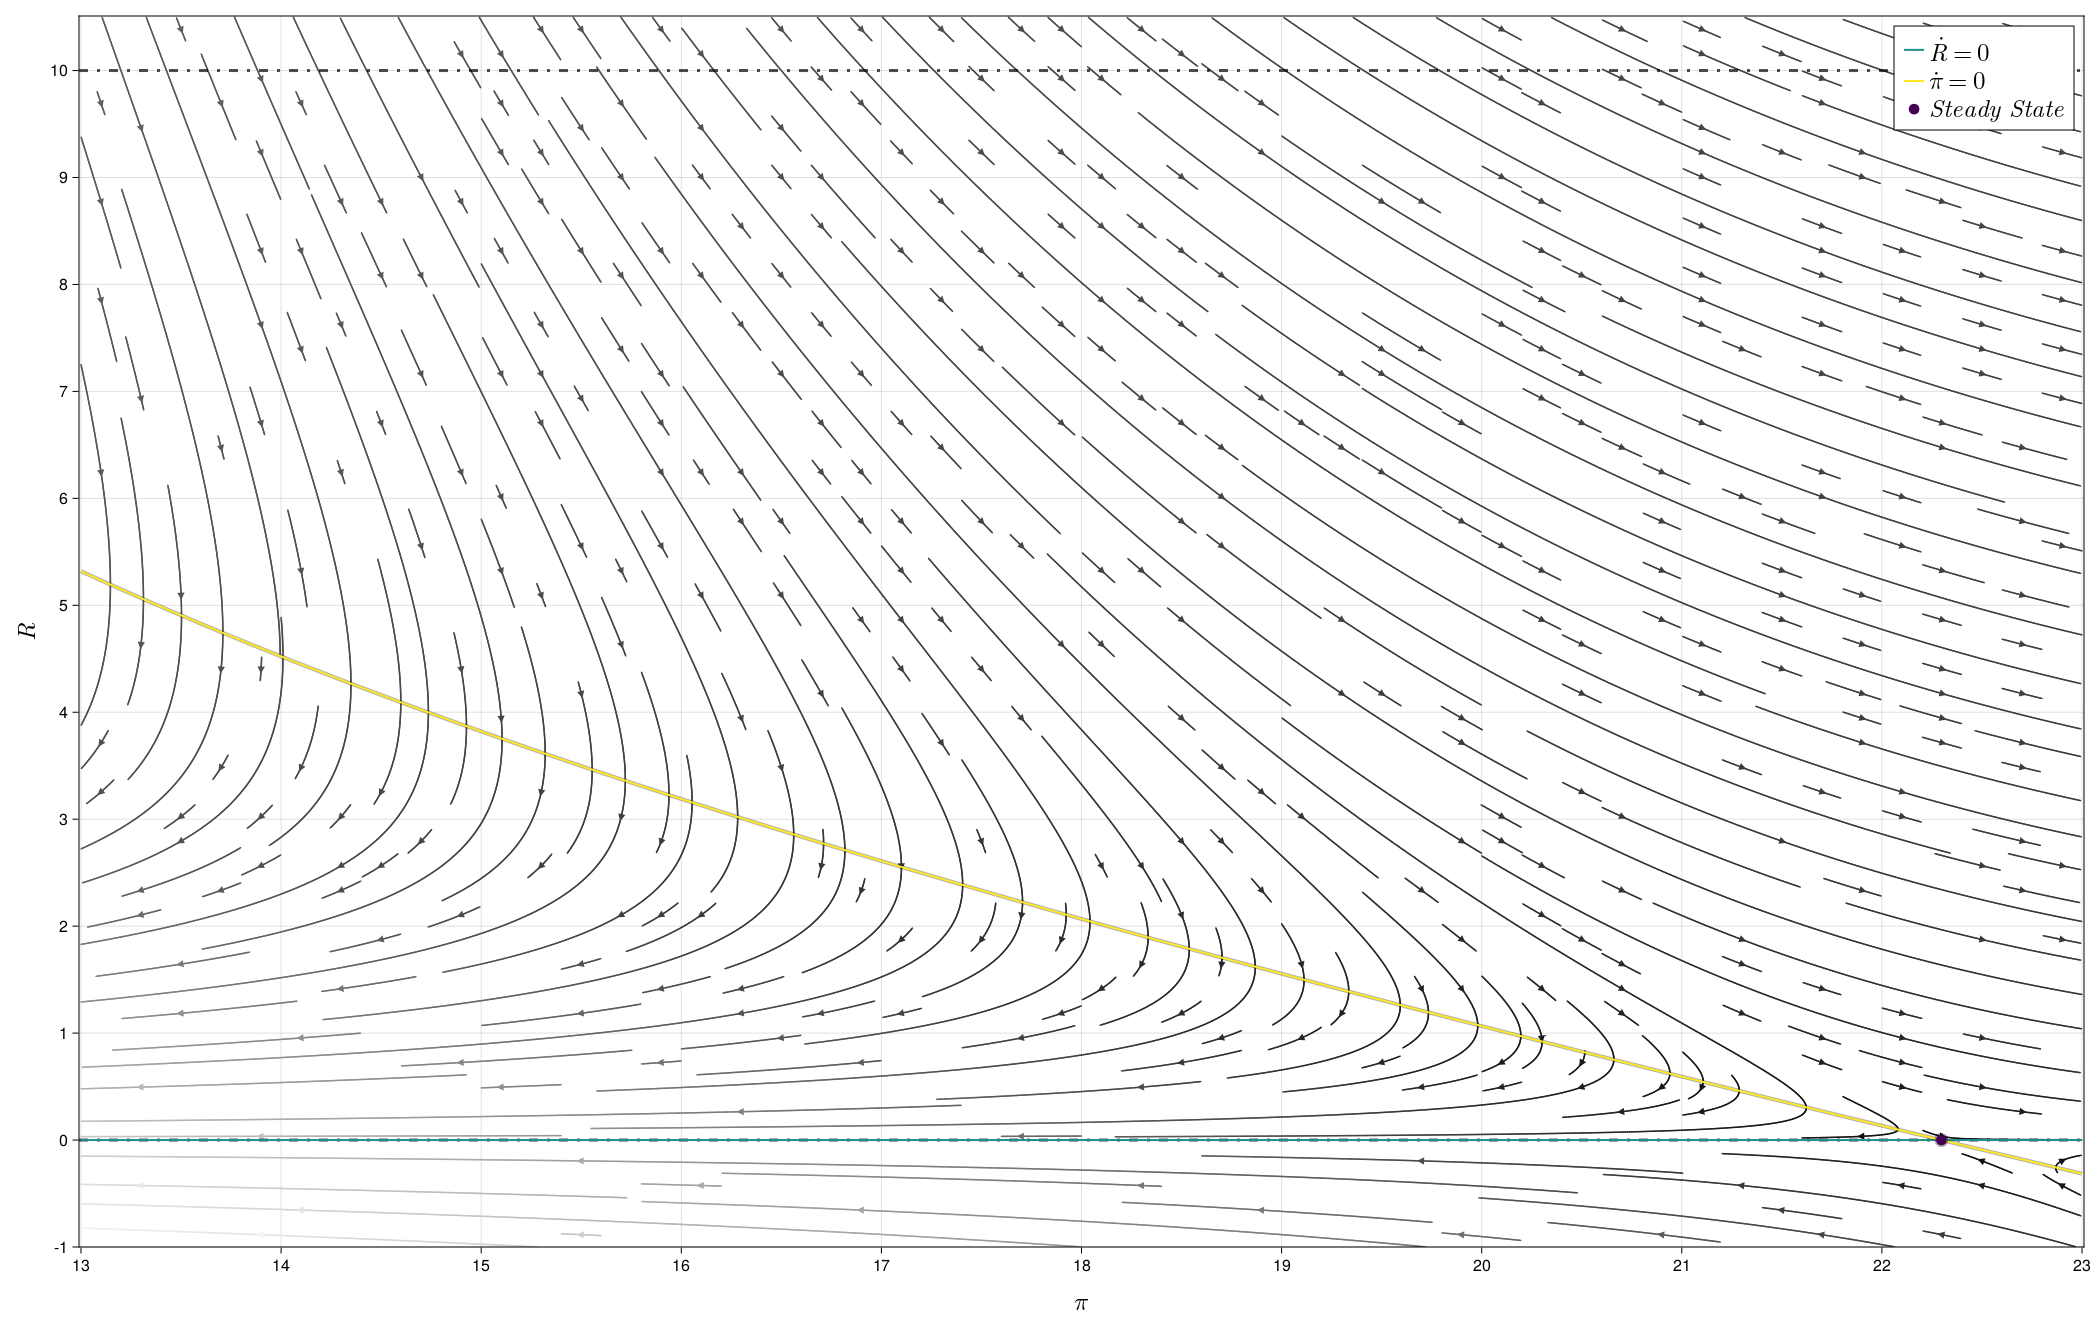
\includegraphics[scale = 0.195]{04_Chapter-3/00A_Figures/Figure_Equilibrium-Path_Endogenous-Price_Phase-Diagram_pi-by-R.png}
        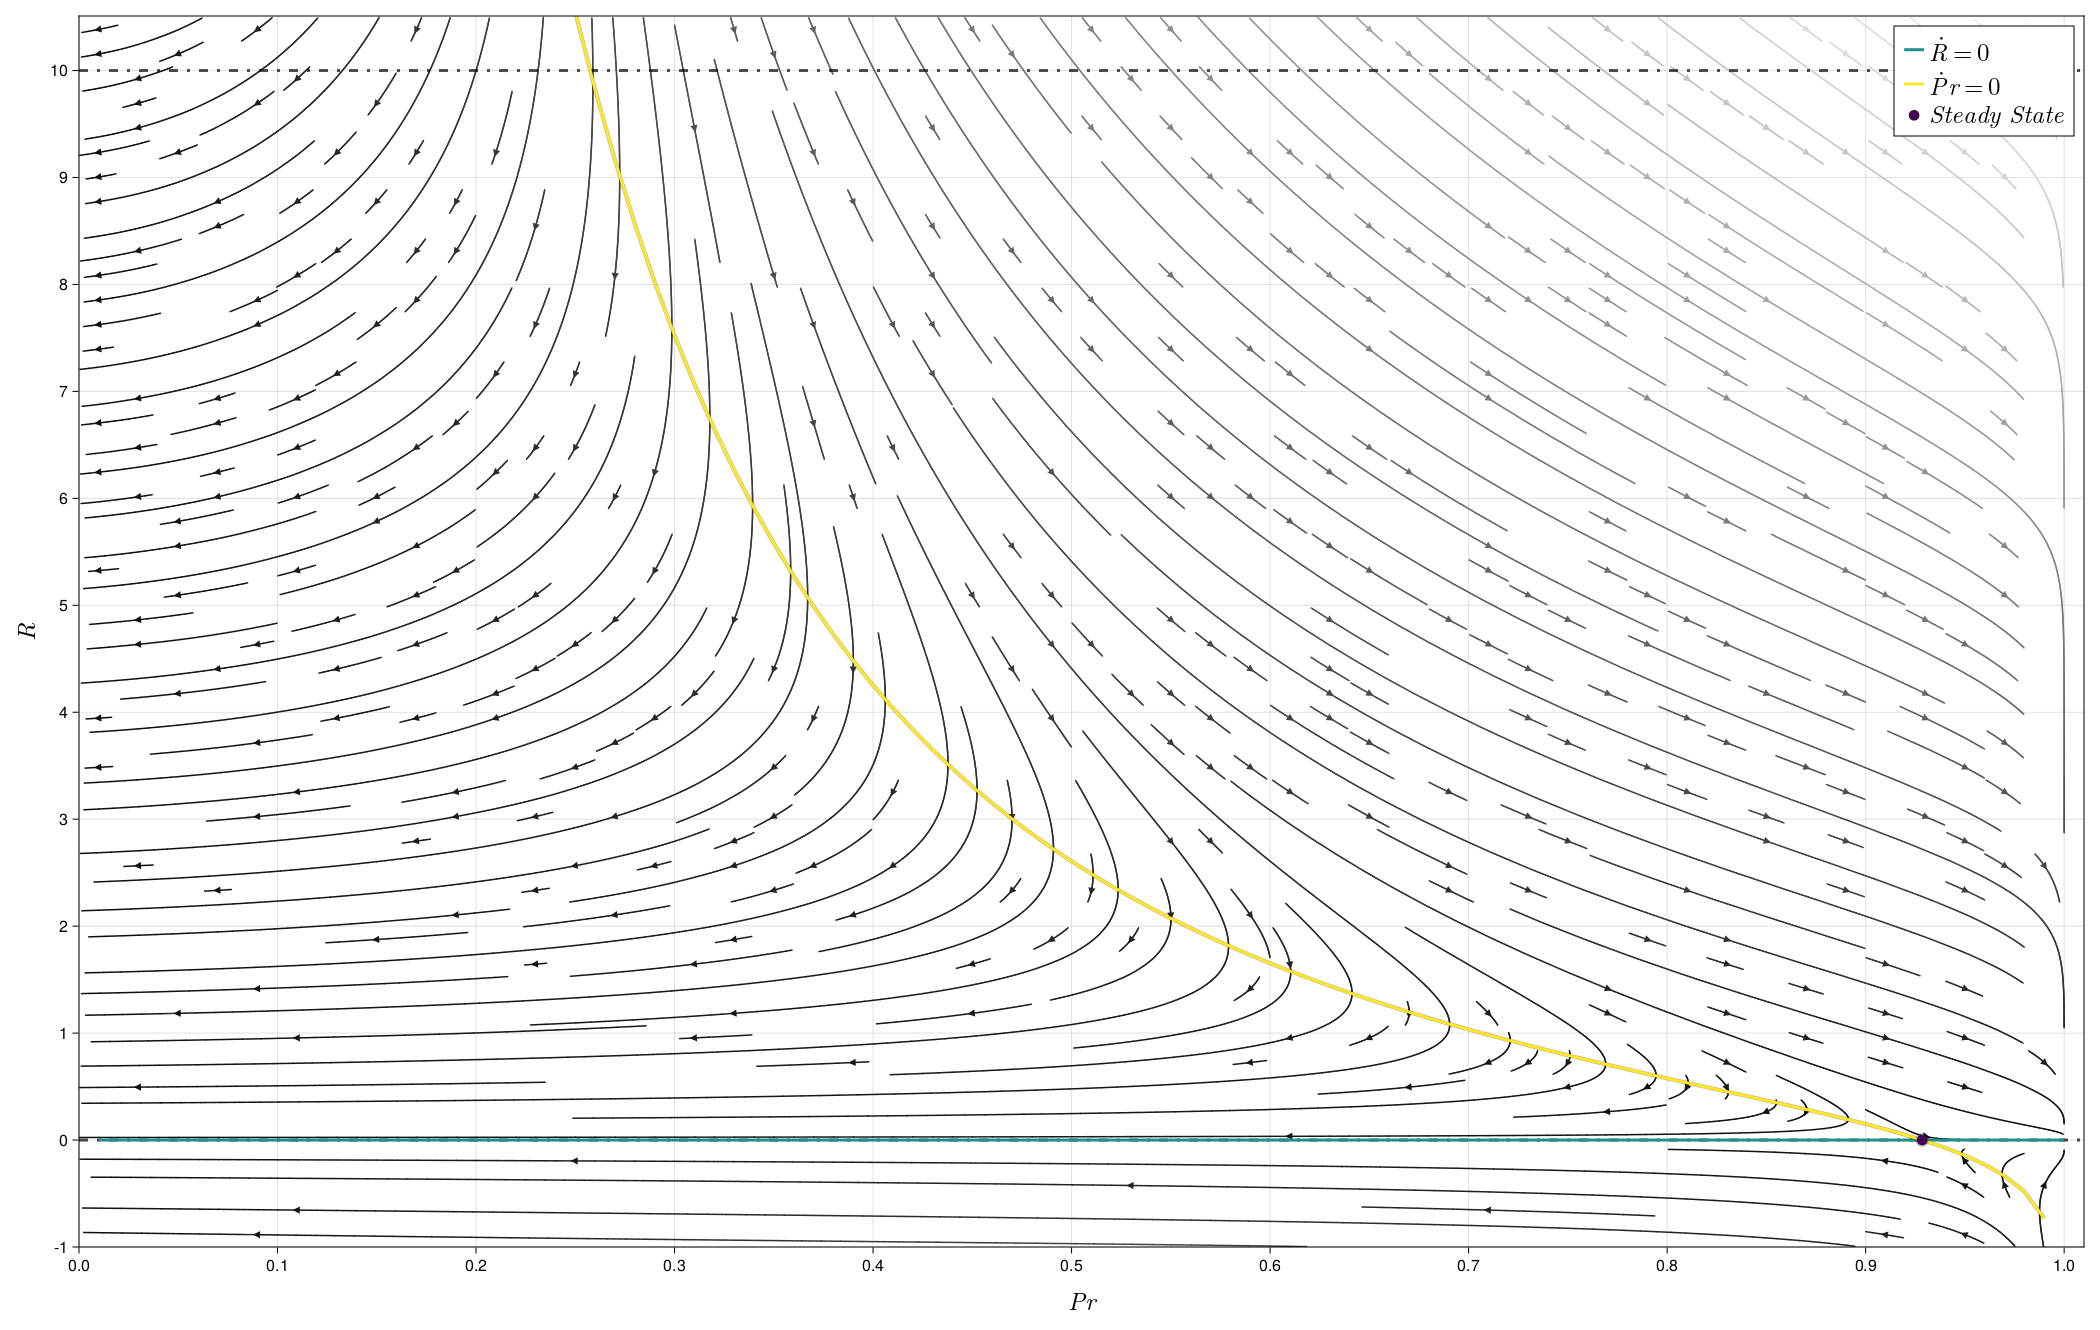
\includegraphics[scale = 0.195]{04_Chapter-3/00A_Figures/Figure_Equilibrium-Path_Endogenous-Price_Phase-Diagram_Pr-by-R.png}
        \caption{Phase Diagrams for the Social Planner's Problem}
        \caption*{
            {\small
            \textit{Note}: 
            This figure demonstrates two phase diagrams for the social planner's problem. The upper diagram illustrates that the steady state is exactly a saddle point. This figure assumes that a dispersion parameter of $\sigma = 1$, an interest rate of $r = 0.15$, an initial number of well sites of $R_{0} = 10$, additional well sites of $E = 0$, and exogenously given constant oil prices of $p = 50$. Also, a linear cost function of $c(D_{t}) = 2D_{t}$ is assumed.  
        }}
        \label{Figure:Phase-Diagram_Saddle-Point}
    \end{figure}
}


\subsubsection{Implications of Necessary Conditions}
\label{C3-SubSubSection:Necessary-Conditions}
Necessary conditions (\ref{Equation:Social-Planners-Problem_Necessary-Conditions_Costate-Variable}) and (\ref{Equation:Social-Planners-Problem_Meaning-of-Costate-Variable}) have important economic implications of the optimal path of well sites' depletion. Firstly, necessary condition (\ref{Equation:Social-Planners-Problem_Meaning-of-Costate-Variable}) directly provides us with what $\pi_{t}$ means. In this condition, the three terms in the curly bracket collectively mean the net benefit from the output (i.e., oil or gas) produced from the marginally drilled well site at time $t$. Of note, the last term among them is the expected value of the marginal well location's cost shock at time $t$ when the firm decides to drill it (i.e., $e(1)$). The remaining term in this condition represents the opportunity cost of drilling the marginal site at time $t$.\footnote{If the firm decides not to drill a horizontal well into the marginal well site, then the expected value of $\epsilon_{0,t}$ conditional on $a_{t} = 0$ (i.e., $e(0)$) is the only gain the firm gets from the decision.} Hence, the necessary condition indicates that the costate variable $\pi_{t}$ implies the net shadow value of the marginally drilled well site in the current-value term at time $t$. 

Necessary condition (\ref{Equation:Social-Planners-Problem_Necessary-Conditions_Costate-Variable}) enables us to understand what $\pi_{t}$ means from a different perspective. We can re-write this necessary condition as follows\footnote{We ignore an arbitrary integration constant $\mathcal{C}$ in the derivation because $\mathcal{C} = 0$ from the fact that $Pr_{t}$ is a constant at the steady state as well as equation (\ref{Equation:Social-Planners-Problem_System-of-Equations-for-Steady-State}).}:
\begin{equation}
\begin{split}
    % \dot{\pi}_{t} \ 
    % & = \ r \pi_{t} \ - \ \sigma \big( \gamma \ + \  \ln(1 - Pr_{t}) \big) \\
    % (\dot{\pi}_{t} \ - \ r\pi_{t}) e^{-rt} \
    % & = \ - \sigma \big( \gamma \ - \ \ln(1 - Pr_{t}) \big) e^{-rt} \\
    % \pi_{t} e^{-rt} \
    % & = \ \int_{t}^{\infty} e^{-r\tau} \sigma \big( \gamma \ - \ \ln(1 - Pr_{\tau}) \big) d\tau \ + \ \mathcal{C} \\  % C = 0 from the equation for \pi_{t} at the steady state.
    \pi_{t} \
    & = \ e^{rt} \left[ \int_{t}^{\infty} e^{-r\tau} \Big\{ f_{t} \ + \ \sigma \big( \gamma \ - \ \ln(1 - Pr_{\tau}) \big) \Big\} d\tau \right],
\end{split}
\label{Equation:Social-Planners-Problem_Euler-Equation}
\end{equation}
This equation implies that $\pi_{t}$ is the marginally undrilled well site's aggregate expected utility (i.e., the sum of the expected value of $\epsilon_{0,t}$'s over time), as the current value at time $t$, if the well site will remain undeveloped. Therefore, it is clear that drilling well locations is economic depletion in our framework, as extracting an exhaustible resource is in Hotelling's model. 

Collectively, necessary conditions (\ref{Equation:Social-Planners-Problem_Necessary-Conditions_Costate-Variable}) and (\ref{Equation:Social-Planners-Problem_Meaning-of-Costate-Variable}) suggest that on the optimal path of drilling, the marginal undeveloped well site will be drilled at time $t$ if the net gains from drilling it at time $t$ equal the undrilled site' aggregate future gains from time $t$. In other words, at the margin, drilling a horizontal well today is an optimal choice for the firm if its value is indifferent to the value of simply holding it forever. Indeed, this implication holds under the Hotelling framework. 

Necessary condition (\ref{Equation:Social-Planners-Problem_Necessary-Conditions_Costate-Variable}) demonstrates significant implications of $\pi_{t}$'s growth over time. We can re-express this condition as follows\footnote{From equation (\ref{Equation:Social-Planners-Problem_Euler-Equation}), $\pi_{t} = e^{rt} \sigma \big( \gamma \ - \ \ln(1 - Pr_{t}) \big) \int_{t}^{\infty} e^{-r\tau} d\tau = \sigma \big( \gamma \ - \ \ln(1 - Pr_{t}) \big) / r$ at the steady state.}:
\begin{equation}
%    \dot{\pi}_{t} \ 
%    & = \ r \pi_{t} \ - \ \sigma \big( \gamma \ + \ \ln(1 - Pr_{t}) \big) \\
    \dot{\pi}_{t} \ = \ r \left\{ \pi_{t} \ - \ \frac{ \ f_{t} \ + \ \lambda_{a} \sigma \big( \gamma \ - \ \ln(1 - Pr_{t}) \big) \ }{r} \right\}.
%    \frac{\dot{\pi_{t}}}{\pi_{t}} \ + \  \frac{\sigma \big( \gamma \ - \ \ln(1 - Pr_{t}) \big)}{\pi_{t}} \ 
%    & = \ r
\label{Equation:Social-Planners-Problem_Growth-Rate-of-Costate-Variable}
\end{equation}
This expression clearly indicates that $\pi_{t}$ grows slower than the rate of interest $r$. The necessary condition also suggests that $\pi_{t}$ increases concavely with $Pr_{t}$ and converges in the limit, unlike the exponential growth of the shadow price on the law of motion in Hotelling's framework.\footnote{From the beginning of drilling (i.e., $t = 0$), $R_{t}$ decreases. If $Pr_{t}$ is maintained at a lower level, the rate of drilling will quickly converge to zero. So, $Pr_{t}$ must continuously grow to keep drilling. In equation (\ref{Equation:Social-Planners-Problem_Growth-Rate-of-Costate-Variable}), $Pr_{t}$'s increase leads to the reduction in $\dot{\pi}_{t}$.} 

The value of $\sigma$, which is the dispersion parameter of the I.I.D. T1EV cost shocks, provides two interesting implications. First, the social planner's problem reverts to the Hotelling model of the optimal extraction of a nonrenewable resource when $\sigma$ goes to zero. Taking limits to zero for necessary conditions (\ref{Equation:Social-Planners-Problem_Necessary-Conditions_Costate-Variable}) and (\ref{Equation:Social-Planners-Problem_Meaning-of-Costate-Variable}) yields the followings, which are identical to the two necessary conditions in Hotelling's classic model of depletion\footnote{In the limiting case, we ignore the flow utility $f_{t}$, which is not introduced in Hotelling's theoretical model.}:
\begin{equation}
\begin{cases}
        \begin{split}
        \ \lim_{\sigma \to 0} \dot{\pi}_{t} \
        & = \ r\pi_{t} \\
        \ \lim_{\sigma \to 0} \pi_{t} \
        & = \ \alpha u'(\alpha R_{t} Pr_{t}) \ - \ c'(R_{t} Pr_{t}).
        \end{split}
    \end{cases}
\label{Equation:Social-Planners-Problem_Reverting-to-the-Hotelling-Model}
\end{equation}
Intuitively, the limiting case that $\sigma$ takes a value of zero means that the drilling decision for the marginal well location depends only on drilling costs and the interest rate $r$, which are not stochastic, unlike cost shocks $\epsilon(a_{t})$'s.

Second, the magnitude of $\sigma$ determines the rate of drilling, and also production. To be specific, an increase in the magnitude of $\sigma$ reduces drilling. When the value of $\sigma$ grows, the importance of the cost shocks increases relative to the observable components in the utility function (i.e., $\tilde{U}(\cdot)$). In other words, as more utility comes from the cost shocks, the option value of each well location increases. Therefore, a larger value of $\sigma$ makes the social planner wait for a better shock, which in turn, delays well drilling. 

Transversality condition (\ref{Equation:Social-Planners-Problem_Transversality-Condition}) rules out too aggressive depletion of well sites. Note that the transversality condition holds even when $R_{t} \neq 0$.


% Firm's Problem
\subsection{Firm's Problem}
\label{C3-SubSection:Firms-Problem}
In this section, we develop the firm's problem under the settings of our DCDP model in continuous time. We first introduce additionally required building blocks. In particular, we integrate heterogeneity in the quality of well sites into the problem. Following \cite{Estimation-of-Dynamic-Discrete-Choice-Models-in-Continuous-Time_ABBE_2016}, we formulate the value function for a given well site. And then, utilizing the value function, we show that the oil market clears. In addition, we formulate firm-level optimal paths by aggregating the firm's well-level drilling decisions. 

\subsubsection{Firm's Decisions on Drilling Well Sites}
\label{C3-SubSubSection:Firms-Decisions-on-Drilling-Well-Sites}
In our formulation, a particular well site $i$ can be in state $k$ at some time $t$. This $k$ is an integer scalar index $k = 1, 2, \cdots, K$, by which every available state in a finite state space $\mathcal{X}$ is enumerated.\footnote{As implied, $\mathcal{X}$ is a discrete state space.} For simplicity, it is assumed that the firm can drill only one horizontal well in that well location $i$. 

Exploiting the same index system, we discretize oil prices that are a state variable in the firm's problem. Specifically, for a given oil production $Q$, the oil price in state $k$ (denoted $p_{k}$) is determined by the following:
\begin{equation}
\begin{split}
	p_{k} \
	& = \ p_{0,k} \ - \ \widebar{p}_{1} Q.
\end{split}
\label{Equation:Firms-Problem_Oil-Prices}
\end{equation}
where $p_{0,k}$ and $\widebar{p}_{1}$ are non-negative. In our setting, oil prices can vary due to two distinct finite-state Markov jump processes.\footnote{A Markov jump process with finite states is a stochastic process that has discrete movements governed by a Poisson arrival process. For details, see \cite{Time-Discretization-of-Markov-Chains_Doytchinov-and-Irby_2010}.} One is a jump process on $\mathcal{X}$. Parameters $\lambda_{k\ell}$ that indicate the rates at which particular state transitions from $k$ to $\ell \neq k$ occur govern this process. The firm's actions, following a Poisson arrival process with rate parameter $\lambda_{a}$, drive the other process. Specifically, when the firm chooses the action $a = 1$, which means drilling a horizontal well in site $i$, from the discrete choice set $\mathcal{A} = \{ 0, 1 \}$, $p_{\ell(i, a, k)}$ is the price in the resulting state $\ell(i, a, k)$.\footnote{This implicitly assumes that oil prices are determined endogenously and that the firm takes oil prices as given in a competitive equilibrium.}\footnote{$a = 0$ is a costless continuation choice.}

The firm, which is forward-looking and discounts future payoffs at rate $\rho \in (0, \infty)$, receives two different types of payoffs. First, the firm receives flow payoff with respect to a particular undrilled well site $i$ being in state $k$. We formulate the flow payoff $f_{ik}$ as a function of oil prices: $f_{ik} (p_{k}; \boldsymbol{\theta_{f}})$.\footnote{In this formulation, $\boldsymbol{\theta}_{f}$ is a vector of parameters, which depends on a specific functional form.} Here, we assume that the firm exits the market after drilling a horizontal well into the site $i$. In other words, the firm gets no flow payoff from well locations already drilled. 

Regarding a given well site $i$ in state $k$, the firm also receives an instantaneous payoff when taking action $a \in \mathcal{A}$. This choice-dependent payoff consists of a choice-specific payoff $\psi_{iak}$ and a choice-specific payoff shock $\epsilon_{iak}$, which is observable only to the firm. We formulate the choice-specific payoff as follows:
\begin{equation}
\begin{split}
%    \psi_{iak}(\boldsymbol{x}_{ik}, a; \boldsymbol{\theta}_{\psi}) \
    \psi_{iak}(p_{k}, a; \boldsymbol{\theta}_{\psi}) \
    & = \ 
    \begin{cases}
        \ \alpha p_{k} \ - \ c \hspace{0.5cm} \text{if \ $a = 1$} \\
        \ 0 \hspace{1.8cm} \text{otherwise},
%        \ \big\{ g_{i}^{L} \ + \ (1 - g_{i}^{L}) \alpha^{H} \big\} p_{k} \ - \ c \hspace{0.5cm} \text{if $s_{ik} = 0$ and $a = 1$} \\
%        \ 0 \hspace{4.65cm} \text{otherwise},
    \end{cases}
\end{split}
\label{Equation:Firms-Problem_Instantaneous-Payoff}
\end{equation}
where $\boldsymbol{\theta}_{\psi}$, which is a vector of parameters, consists of two elements: $\alpha$ is the normalized oil production from the site $i$, whereas $c$ stands for drilling costs.\footnote{That is, $\boldsymbol{\theta}_{\psi} = (\alpha, c)$.} Clearly, for a given undrilled well site $i$, the firm gets an instantaneous payoff $\psi_{iak} + \epsilon_{iak}$, whose value varies with the firm's choice $a \in \mathcal{A}$. And the firm gets no instantaneous payoff from already drilled sites. Here, we assume that the $\epsilon_{iak}$'s are I.I.D. and follow $T1EV(0, \sigma)$. 

In our continuous-time framework, the value function for a particular well site $i$ in state $k$ is given as follows\footnote{Detailed derivation is presented in \ref{C3-Appendix_Derivations_Value-Function-in-Continuous-Time}.}:
\begin{equation}
\begin{split}
    % \left( \rho \ + \ \sum_{\ell \neq k} \lambda_{k\ell} \ + \ \lambda_{d} \right) V_{ik} \ 
    % & = \ f_{ik} \ + \ \sum_{\ell \neq k} \lambda_{k\ell} V_{i\ell} \ + \ \lambda_{d} E\bigg[ \underset{a}{\max} \left\{ V_{i,\ell(i, a, k)} \ + \ \psi_{iak} \ + \ \epsilon_{iak} \right\} \bigg].
    V_{ik} \ 
    & = 
    \ \frac{
        \ f_{ik} \ + \ \sum_{\ell \neq k} \lambda_{k\ell} V_{i\ell} \ + \ \lambda_{a} E\Big[ \underset{a \in \mathcal{A}}{\max} \left\{ V_{i,\ell(i, a, k)} \ + \ \psi_{iak} \ + \ \epsilon_{iak} \right\} \Big] \ 
    }{
        \rho \ + \ \sum_{\ell \neq k} \lambda_{k\ell} \ + \ \lambda_{a}
    }.
\end{split}
\label{Equation:Firms-Problem_Value-Function}
\end{equation}
Here, the value function $V_{ik}$ represents the present discounted value of all payoffs obtained from starting at state $k$ and behaving optimally in all subsequent periods. $\dot{V}_{ik}$ is the time derivative of $V_{ik}$. The three terms in the round bracket on the left-hand side are the sum of the discount factor and the rates of all possible (i.e., exogenous as well as endogenous) state changes. The right-hand side consists of the flow payoffs, the expected values relying on the firm's decisions, and the rate-weighted values related to exogenous state transitions. The expectation is for the joint distribution of $\epsilon_{i0k}$ and $\epsilon_{i1k}$. $\tilde{f}_{ik}$ and $\tilde{\psi}_{iak}$ indicate payoff changes due to state transitions as a result of the firm's decisions. 

For a given opportunity to choose an action $a \in \mathcal{A}$, the probability of drilling a horizontal well conditional on state $k$, denoted $Pr_{k}$, can be defined as follows\footnote{For given values of parameters, we can compute the value of each $Pr_{k}$, $k = 1, 2, \cdots, K$, by using value function iterations.}:
\begin{equation}
\begin{split}
	Pr_{k} \
	& \equiv \ \Pr \big[ \ \psi_{i1k} + \epsilon_{i1k} \ \geq \ V_{i,\ell(i,0,k)} + \psi_{i0k} + \epsilon_{i0k} \ | \ k \ \big].
\end{split}
\label{Equation:Firms-Problem_CCP}
\end{equation}
From this definition, the hazard rate of action $a$ is $h_{ak} = \lambda_{a} Pr_{k}$. 
As shown in \cite{Estimation-of-Dynamic-Discrete-Choice-Models-in-Continuous-Time_ABBE_2016}, for each action $a \in \mathcal{A}$, the third term in the numerator of equation (\ref{Equation:Firms-Problem_Value-Function}) is the following:
\begin{equation}
\begin{split}
	& E\Big[ \underset{a \in \mathcal{A}}{\max} \left\{ V_{i,\ell(i, a, k)} \ + \ \psi_{iak} \ + \ \tilde{\psi}_{iak} \ + \ \epsilon_{iak} \right\} \Big] \\
	& = \ 
	\begin{cases}
		V_{ik} \ + \ \sigma \big( \gamma \ - \ \ln(1 - Pr_{k}) \big) \hspace{1.6cm} \text{if \ \ $a = 0$} \\
		\psi_{i1k} \ + \ \tilde{\psi}_{i1k} \ + \ \sigma \big( \gamma \ - \ \ln(Pr_{k}) \big) \hspace{0.7cm} \text{if \ \ $a = 1$}.
	\end{cases}
\end{split}
\label{Equation:Firms-Problem_Emax}
\end{equation}

In the case in which the oil price remains constant at $\widebar{p}$, some algebraic manipulation on the value function (\ref{Equation:Firms-Problem_Value-Function}), with the expressions in (\ref{Equation:Firms-Problem_Emax}), yields the Euler equation that drives the dynamics of the firm's optimal drilling decisions\footnote{In our setting, constant oil price implies no state transition.}:
\begin{equation}
\begin{split}
    % (\rho \ + \ \lambda_{a}) V_{ik} \
    % & = \ f_{ik} \ + \ \lambda_{a} \left\{ \psi_{i1k} \ + \ \sigma \big( \gamma \ - \ \ln(Pr_{k}) \big) \right\} \\
    % (\rho \ + \ \lambda_{a}) \cdot \frac{1}{\rho} \left\{ f_{ik} \ + \ \lambda_{a} \sigma \big( \gamma \ - \ \ln(1 - Pr_{k}) \big) \right\} \
    % & = \ f_{ik} \ + \ \lambda_{a} \left\{ \psi_{i1k} \ + \ \sigma \big( \gamma \ - \ \ln(Pr_{k}) \big) \right\} \\
    % (\rho \ + \ \lambda_{a}) \left\{ f_{ik} \ + \ \lambda_{a} \sigma \big( \gamma \ - \ \ln(1 - Pr_{k}) \big) \right\} \
    % & = \ \rho f_{ik} \ + \ \rho \lambda_{a} \left\{ \psi_{i1k} \ + \ \sigma \big( \gamma \ - \ \ln(Pr_{k}) \big) \right\} \\
    % \lambda_{a} f_{ik} \ + \ (\rho \ + \ \lambda_{a}) \lambda_{a} \sigma \big( \gamma \ - \ \ln(1 - Pr_{k}) \big) \
    % & = \ \rho \lambda_{a} \left\{ \psi_{i1k} \ + \ \sigma \big( \gamma \ - \ \ln(Pr_{k}) \big) \right\} \\
    % f_{ik} \ + \ (\rho \ + \ \lambda_{a}) \sigma \big( \gamma \ - \ \ln(1 - Pr_{k}) \big) \
    % & = \ \rho \left\{ \psi_{i1k} \ + \ \sigma \big( \gamma \ - \ \ln(Pr_{k}) \big) \right\} \\
    % f_{ik} \ + \ \lambda_{a} \sigma \big( \gamma \ - \ \ln(1 - Pr_{k}) \big) \
    % & = \ \rho \left\{ \psi_{i1k} \ + \ \sigma \big( \gamma \ - \ \ln(Pr_{k}) \big) \ - \ \sigma \big( \gamma \ - \ \ln(1 - Pr_{k}) \big) \right\} \\
    \frac{ \ f_{ik} \ + \ \lambda_{a} \sigma \big( \gamma \ - \ \ln(1 - Pr_{k}) \big) \ }{\rho} \
    & = \ \left\{ \psi_{i1k} \ + \ \sigma \big( \gamma \ - \ \ln(Pr_{k}) \big) \right\} \ - \ \sigma \big( \gamma \ - \ \ln(1 - Pr_{k}) \big).
\end{split}
\label{Equation:Firms-Problem_Euler-Equation}
\end{equation}
In this equation, the left-hand side represents the firm's payoff when deciding not to drill a horizontal well in state $k$. In other words, the left-hand side is the payoff for the case that the firm chooses $a = 0$ at a decision point and remains in state $k$. The right-hand side is the firm's payoff if it chooses to drill a horizontal well into well site $i$. Importantly, it is evident that equation (\ref{Equation:Firms-Problem_Euler-Equation}) drawn from the firm's well-level decisions coincides with necessary condition (\ref{Equation:Social-Planners-Problem_Meaning-of-Costate-Variable}) of the social planner's problem.\footnote{The only difference is $\lambda_{a}$ on the left-hand side in equation (\ref{Equation:Firms-Problem_Euler-Equation}), which governs how often the firm makes decisions of whether or not to drill a given well site.}


\subsubsection{Aggregation of Well-Level Drilling Decisions}
\label{C3-SubSubSection:Aggregation-of-Well-Level-Drilling-Decisions}
\textit{\textbf{The Firm's (Expected) Payoff Maximization Problem}} ---
The firm aims to maximize the total payoffs from drilling its well sites. Because the instantaneous payoff includes choice-dependent shocks $\epsilon_{iak}$, which follow the distribution of $TIEV(0, \sigma)$, the payoff the firm receives when drilling an individual well site $i$ is an expected value. So, the firm's problem is given by
\begin{footnotesize}
\begin{equation}
\begin{split}
    \underset{\{Pr_{t}\}_{t = 0}^{\infty}}{\max} \hspace{0.1cm} \int_{0}^{\infty} e^{-\rho t} \sum_{g \in \mathcal{Q}} R_{t}^{g} \left[ f_{t}^{g} \ + \ \lambda_{a} \Big\{ Pr_{t}^{g} \cdot \Big( \psi_{t}^{g} \ + \ \sigma \big( \gamma - \ln(Pr_{t}^{g}) \big) \Big) \ + \ (1 - Pr_{t}^{g}) \cdot \sigma \big( \gamma - \ln(1 - Pr_{t}^{g}) \big) \Big\} \right] dt
\end{split}
\label{Equation:Firms-Problem_Expected-Payoff-Maximization-Problem}
\end{equation}
\end{footnotesize}
subject to
\begin{equation}
\begin{split}
    \dot{R}_{t}^{g} \ = \ -R_{t}^{g} \big( \lambda_{a} Pr_{t}^{g} \big) \ + \ E^{g}, \hspace{0.3cm} R_{0}^{g} \ = \ R^{g}(0) \ = \ 1 \hspace{0.2cm} \text{given,}
\end{split}
\end{equation}
\begin{equation}
\begin{split}
    R_{t}^{g} \ \geq \ 0, \hspace{0.3cm} 0 \leq \ Pr_{t}^{g} \ \leq \ 1.
\end{split}
\end{equation}
As shown, we normalize the low- and high-quality reserves of well sites to 1. In this formulation, $\lambda_{a} Pr_{t}^{g} \hspace{0.15cm} (\equiv h_{t}^{g})$ means the hazard rate of drilling at time $t$. 

When the firm is drilling (i.e., $R_{t}^{g} > 0$ and $Pr_{t}^{g} \in (0, 1)$), the necessary conditions of the Hamiltonian-Lagrangian for the firm's problem are as follows\footnote{The Hamiltonian-Lagrangian of the firm's problem is presented in \ref{C3-Appendix_Derivations_Firms-Problem_Necessary-Conditions}.}:
\begin{equation}
\begin{split}
    & R_{t} \lambda_{a} \big\{ \psi_{t}^{g} - \ \sigma \ln(Pr_{t}^{g}) \ + \ \sigma \ln(1 - Pr_{t}^{g}) \ - \ \pi_{t}^{g} \big\} \ - \ \lambda_{2,t} \ + \ \lambda_{3,t} \ \leq \ 0, \hspace{0.2cm} Pr_{t}^{g} \ \geq \ 0,  \hspace{0.2cm} \text{C.S.},
\end{split}
\label{Equation:Firms-Problem_Necessary-Conditions_Drilling-Probability}
\end{equation}
\begin{equation}
\begin{split}
    \dot{\pi}_{t}^{g} \ 
    & = \ r \pi_{t}^{g} \ - \ \big\{ f_{t}^{g} \ + \ \lambda_{a} \sigma \big( \gamma \ - \ \ln(1 - Pr_{t}^{g}) \big) \big\} \ - \ \lambda_{1,t},
\end{split}
\label{Equation:Firms-Problem_Necessary-Conditions_Costate-Variable}
\end{equation}
\begin{equation}
\begin{split}
    \lim_{t \rightarrow \infty} e^{-rt} (R_{t}^{g} \pi_{t}^{g}) \ = \ 0.
\end{split}
\label{Equation:Firms-Problem__Transversality-Condition}
\end{equation}
With some algebra and the assumption of no exogenous price change, the necessary conditions (\ref{Equation:Firms-Problem_Necessary-Conditions_Drilling-Probability}) and (\ref{Equation:Firms-Problem_Necessary-Conditions_Costate-Variable}) yields the equation (\ref{Equation:Firms-Problem_Euler-Equation}).\footnote{The derivation details are described in \ref{C3-Appendix_Derivations_Euler-Equation-for-the-Firms-Problem}. In this optimization problem, we can think that $Pr_{t}$ at time $t$ takes one of $Pr_{k}$, $k = 1, 2, \cdots, K$, where $K$ is an arbitrary very large integer.}  Importantly, the identical equation in both optimization levels suggests that the firm's optimal drilling decision for a particular well site $i$ leads to the optimal drilling path at the firm level. 


\par
\vspace{0.3cm}
\noindent
\textit{\textbf{Aggregate Drilling and Production}} ---
For the firm's reserves of well sites with a specific quality $g \in \mathcal{Q}$, the drilling and production are as follows:
\begin{equation}
\begin{cases}
    \begin{split}
        D_{t}^{g} \
        & = \ R_{t}^{g} h_{t}^{g} \hspace{0.2cm} (= -\dot{R}_{t}^{g} \ + \ E^{g}) \\
        Q_{t}^{g} \
        & = \ \alpha^{g} D_{t}^{g}.
    \end{split}
\end{cases}
\label{Equation:Firms-Problem_Aggregate-Drilling-and-Production}
\end{equation}
Therefore, the firm's aggregate drilling and production are simply the sum of drilling and production over different grades. 

The equations for aggregate drilling and production imply two interesting points. First, $D_{t}^{g}$ converges to $E^{g}$ as time goes by, which implies no change in the amount of the remaining reserves, because $\lim_{t \to \infty} R_{t}^{g} = E^{g} / h_{t}^{g}$.\footnote{With some algebra, we find that $R_{t}^{g} = E^{g}/h_{t}^{t} \ + \ (R_{0}^{g} - E^{g}/h_{t}^{g}) e^{-h^{g} t}$.} Second, the firm puts more weight on developing high-quality well locations.\footnote{The reason for this is $Pr_{t}^{H} > Pr_{t}^{L}$, which is true because $\psi_{1k}^{H} > \psi_{1k}^{L}$ in the second line of equation (\ref{Equation:Firms-Problem_Euler-Equation}).} In other words, per-drilling oil production decreases as time $t$ goes to infinity. 

